% DO NOT COMPILE THIS FILE DIRECTLY!
% This is included by the other .tex files.

\begin{frame}
\titlepage
\end{frame}


\section{What has happened since the last MUG}

\section{Give you a brief update over the highlights}

\begin{frame}
  \frametitle{A topical listing of the new major features}
  \begin{itemize}
      \item {\bf Workflow} improvements
      \item {\bf STIX 2.1} improvements along with TAXII integration
      \item {\bf Freetext} import modernisation
      \item {\bf Logging} and {\bf security} improvements
      \item {\bf Dashboard} rework
      \item {\bf Security fixes} and other improvements
  \end{itemize}
\end{frame}


\begin{frame}
  \frametitle{Workflows}
  \begin{itemize}
     \item Continuous ongoing work
     \item Further addition of {\bf logic nodes} for more advanced {\bf branching} decision trees
     \item Additional {\bf action nodes} (such as e-mailing improvements)
     \item The inclusion of new {\bf triggers} based on community feedback
     \item {\bf Filtered data} paths within workflows (e.g. Only execute this set of actions on a subset of the workflow's input data)
  \end{itemize}
\end{frame}

\begin{frame}
\frametitle{Workflows}
\begin{center}
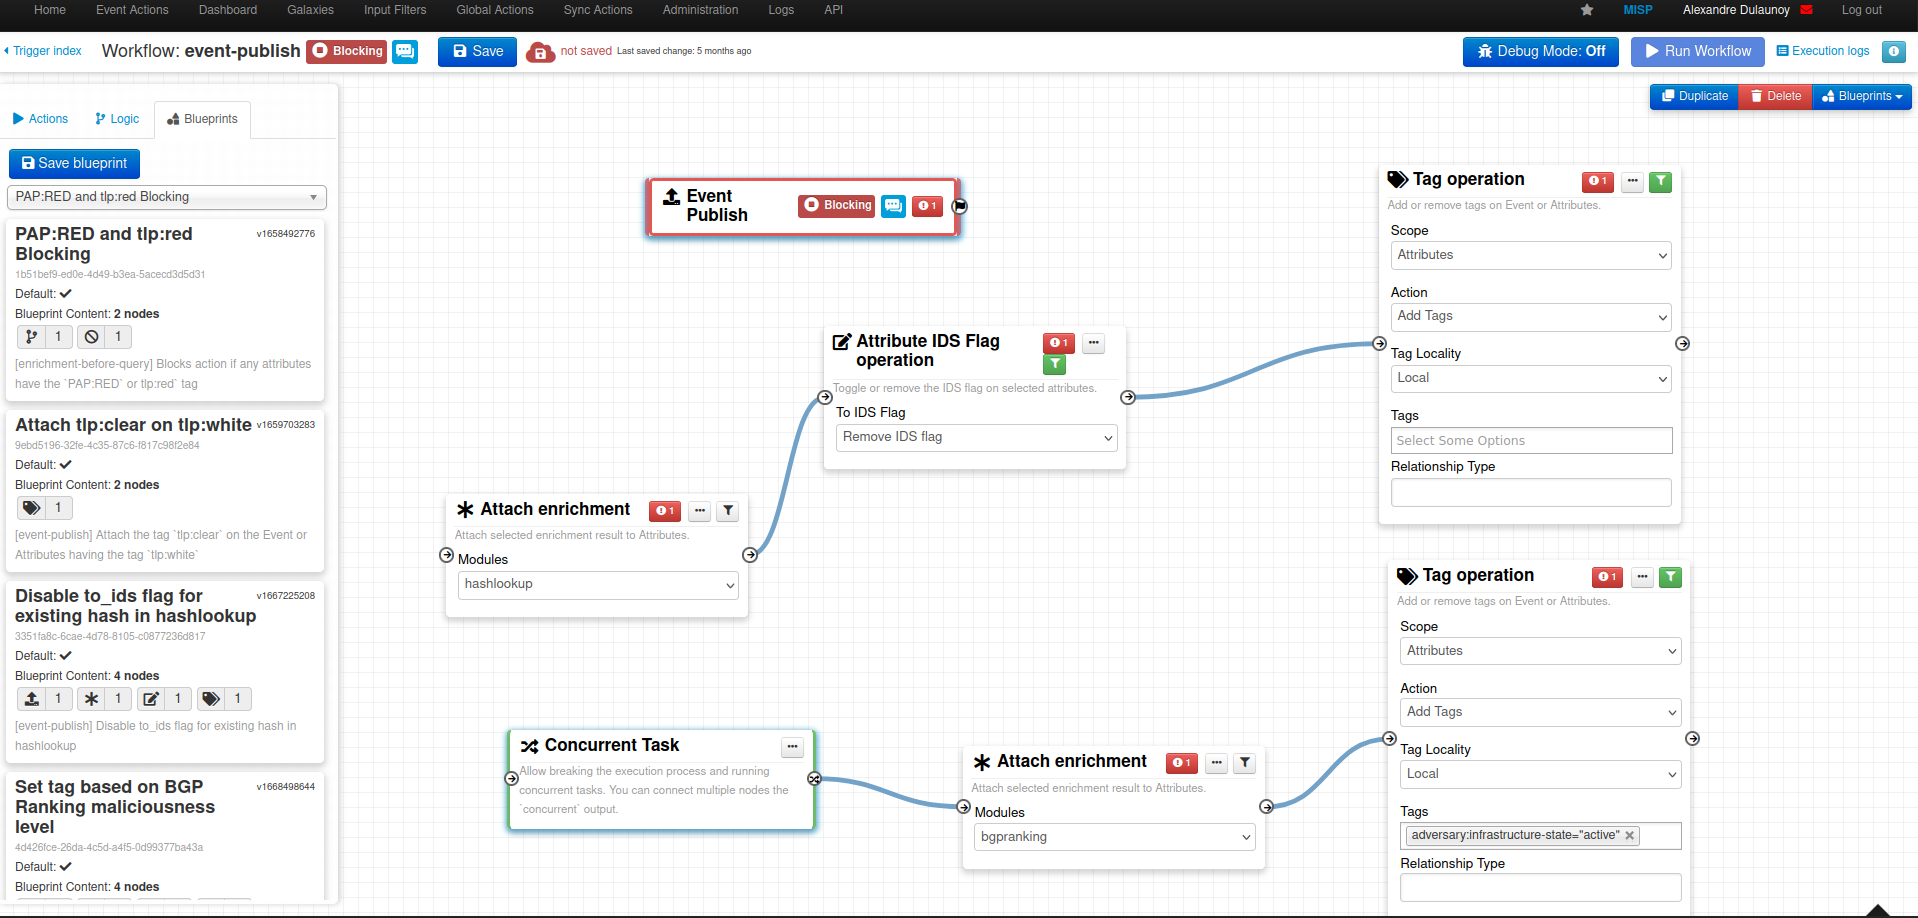
\includegraphics[scale=0.17]{images/workflows_filtered.png}
\end{center}
\end{frame}

\begin{frame}
  \frametitle{Freetext import improvements}
  \begin{itemize}
      \item The {\bf freetext import} has been a powerful way of creating {\bf attributes} parsed out of text
      \item Since 2.4.167, it can also be used to {\bf create MISP objects }
      \item {\bf Proposes} valid object {\bf templates} for the given data-points
      \item New UI elements and parsing logic added
      \item Objects in general encouraged over flat attributes
      \item Goes hand-in-hand with new {\bf object template} development
  \end{itemize}
\end{frame}

\begin{frame}
\frametitle{Freetext import improvements}
\begin{center}
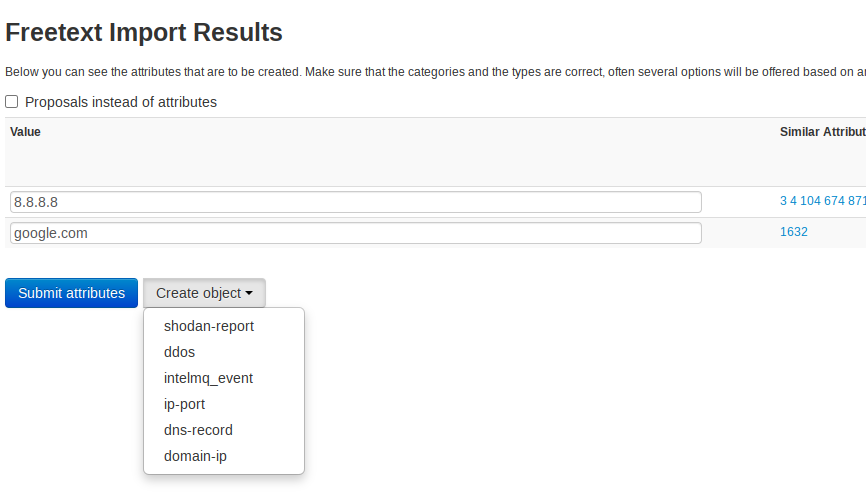
\includegraphics[scale=0.40]{images/freetext_objects.png}
\end{center}
\end{frame}


\begin{frame}
  \frametitle{Logging rework}
  \begin{itemize}
     \item {\bf Logging concerns separated} into optional separate mechanisms
     \begin{itemize}
         \item Separate Application, Audit, Access logs (thanks to Jakub Onderka)
     \end{itemize}
     \item New user sanity checks on {\bf prior authentications} and {\bf associated IPs} (thanks to Christophe Vandeplas)
     \begin{itemize}
         \item Allows users to audit their accounts' actions to catch abuse
     \end{itemize}
     \item New internal logging of {\bf authentication frequency}
  \end{itemize}
\end{frame}

\begin{frame}
  \frametitle{Dashboard rework}
  \begin{itemize}
     \item {\bf Overhaul} of the {\bf widget toolkit} for instance visibility
     \item New widgets to highlight {\bf trends, community interactions and statistics}
     \item Focus on {\bf customisation} and {\bf bucketing} of organisation groups
     \begin{itemize}
         \item Use Organisation meta-data, such as country, sector, org type
     \end{itemize}
     \item Better defined {\bf reporting periods}
     \begin{itemize}
         \item Show data of current day, month, year or since an arbitrary date
     \end{itemize}
     \item Rework of some existing widgets to be much more {\bf performant}
  \end{itemize}
\end{frame}

\begin{frame}

\frametitle{Dashboard example}
\begin{center}
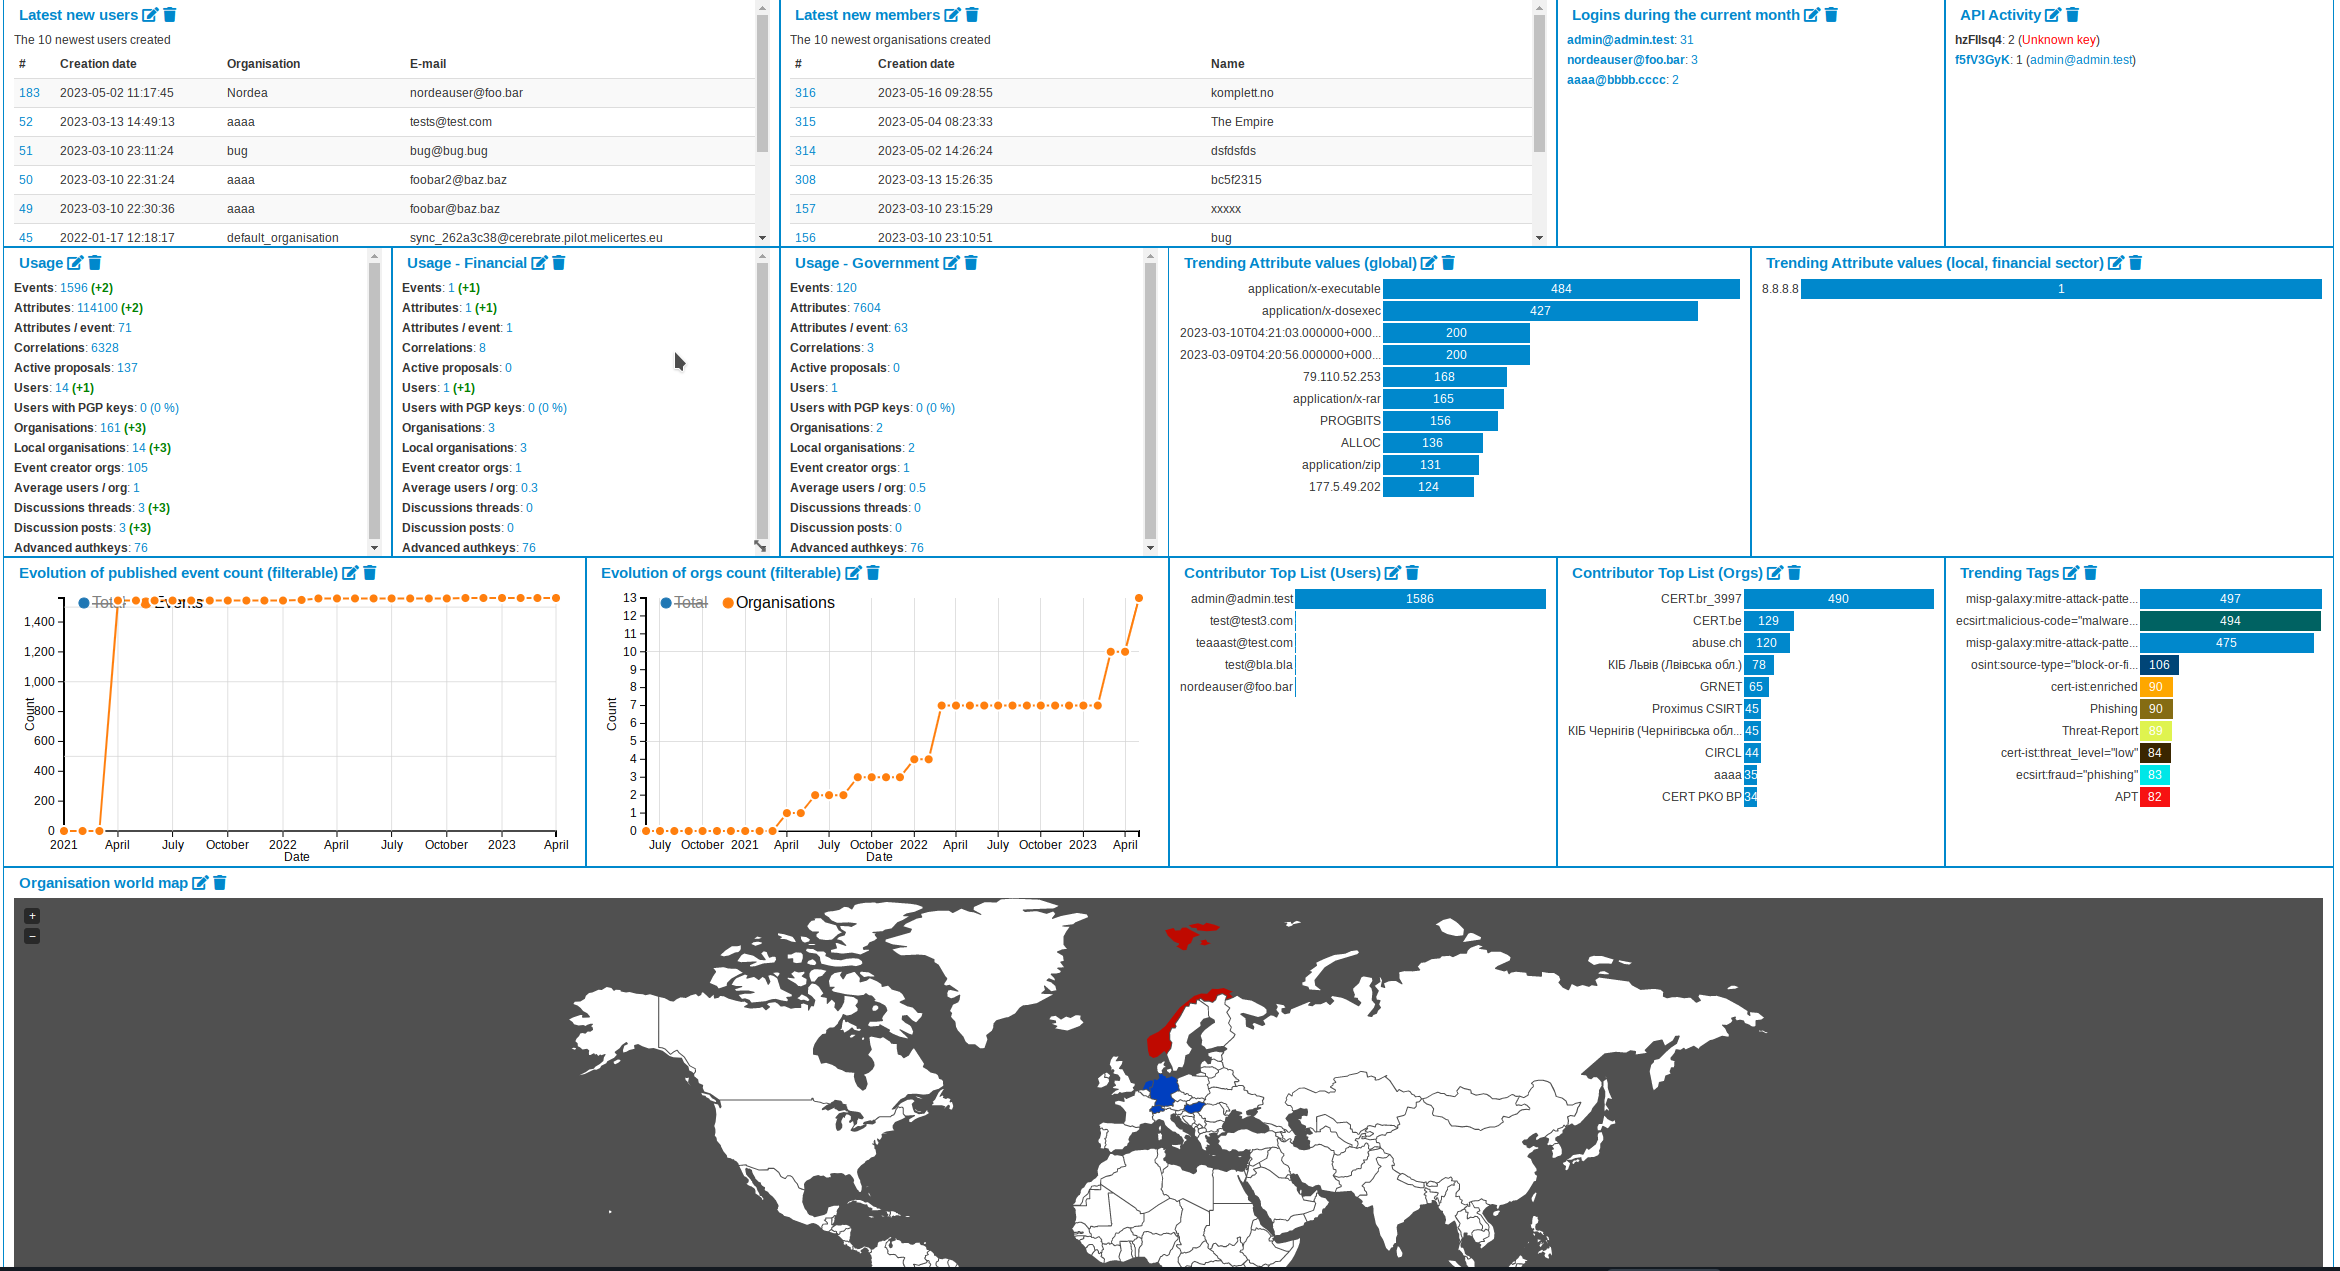
\includegraphics[scale=0.14]{images/dashboard_example.png}
\end{center}
\end{frame}

\begin{frame}
  \frametitle{Security fixes and other improvements}
  \begin{itemize}
     \item Long list of security fixes based on multiple external penetration tests
     \item {\bf CVEs}\footnote{\url{https://www.misp-project.org/security/}} continuously reported for issues small and large
     \begin{itemize}
         \item Make sure you're up to date!
     \end{itemize}
     \item {\bf Zigrin security}'s research funded by the {\bf Luxembourg army} has been a massive help
     \item Long list of other improvements, quality of life changes, performance tuning
  \end{itemize}
\end{frame}

\begin{frame}
\frametitle{Taxonomy highlight}
\begin{itemize}
    \item Many different taxonomies are used frequently in various organisations
    \item A new feature to highlight the important taxonomy in a MISP instance (community) is available
    \item Site admin user can select the {\bf highlighted taxonomies}
    \item The taxonomy namespace will be highlight in a box on the index/event views
\end{itemize}
    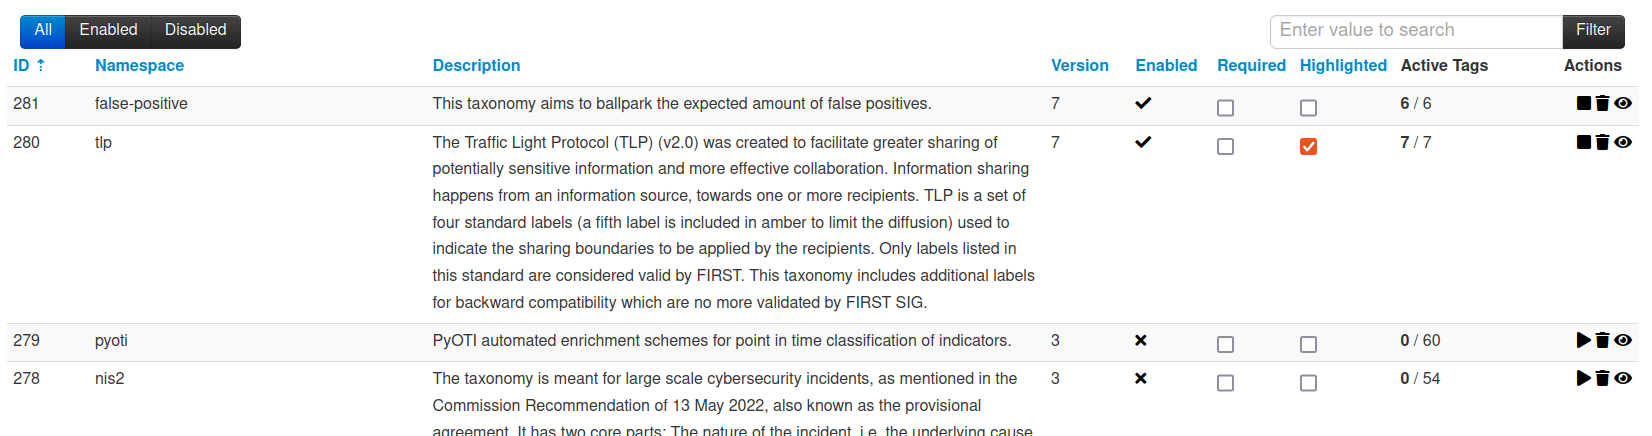
\includegraphics[scale=0.2]{./images/highlight.png}
    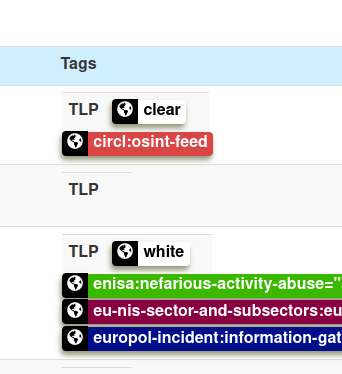
\includegraphics[scale=0.2]{./images/highlight2.png}
\end{frame}

\begin{frame}
\frametitle{MISP modules}
    \begin{itemize}
        \item MISP modules are companion to expansion, export, import for external services or tooling
        \item Extended to support the {\bf MISP workflow actions}
        \item New modules include new import {\bf extract\_url\_components}
        \item New expansion modules include {\bf Crowdsec}, {\bf ipinfo.io}
        \item Improved expansion modules  {\bf greynoise}, {\bf VarIOT}
        \item Improved modules to support the MISP standard format
    \end{itemize}
\end{frame}

\begin{frame}
    \frametitle{MISP taxonomies}
    \begin{itemize}
        \item 149 ready-to-use are now available in MISP taxonomies (used in MISP and many other tools)
        \item New {\bf information-origin} taxonomy to classify AI-generated content with LLMs
        \item New {\bf aviation} taxonomy developed by Eurocontrol to support labelling in the aviation sector
        \item New Microsoft {\bf sentinel} taxonomy to support the MISP sentinel integration developed by Koen Van Impe
        \item Various fixes and improvement to taxonomies (e.g. the dark-web taxonomy due to updates in AIL 5.0)
    \end{itemize}
\end{frame}

\begin{frame}
    \frametitle{MISP warning-lists}
    \begin{itemize}
        \item New {\bf captive-portal} warning-list added
        \item New known {\bf parking page infrastructure} warning-list added 
        \item New {\bf google-chrome-crux-1million} warning-list added
        \item New {\bf microsoft-azure-appid} warning-list added
    \end{itemize}
\end{frame}

\begin{frame}
    \frametitle{MISP galaxy}
    \begin{itemize}
        \item New {\bf sigma} galaxy added including relationships
        \item Latest MITRE ATT\&CK version 13 updated for the MISP galaxy
        \item New microsoft threat actor taxonomy added including relationships with previous activity group and {\bf threat-actor galaxy}
        \item Alignment of {\bf ransomware galaxy} with the {\bf ransomlook.io} project
        \item Major improvements in threat-actor galaxy including relationships with other galaxy clusters
    \end{itemize}
\end{frame}

\begin{frame}
    \frametitle{MISP objects}
\end{frame}

\begin{frame}
     \frametitle{MISP stix}
     \begin{itemize}
        \item misp-stix\footnote{\url{https://github.com/MISP/misp-stix}} is standalone Python library support MISP standard format and all the STIX version (1.1.1, 1.2, 2.0 and 2.1)
        \item Two people from CIRCL are {\bf co-sharing the OASIS Cyber Threat Intelligence (CTI) TC and CTI STIX subcommittee}
        \item Ensuring alignment between the standards, interoperability and an open source standard library
     \end{itemize}
\end{frame}

\begin{frame}
     \frametitle{MISP stix - Custom Galaxy Cluster Import}
     \begin{itemize}
	\item TTPs, Threat Actors and other contextual descriptions imported as Galaxy Clusters
	\item Generating specific Custom Galaxy Clusters from STIX directly
     \end{itemize}
     \begin{center}
	  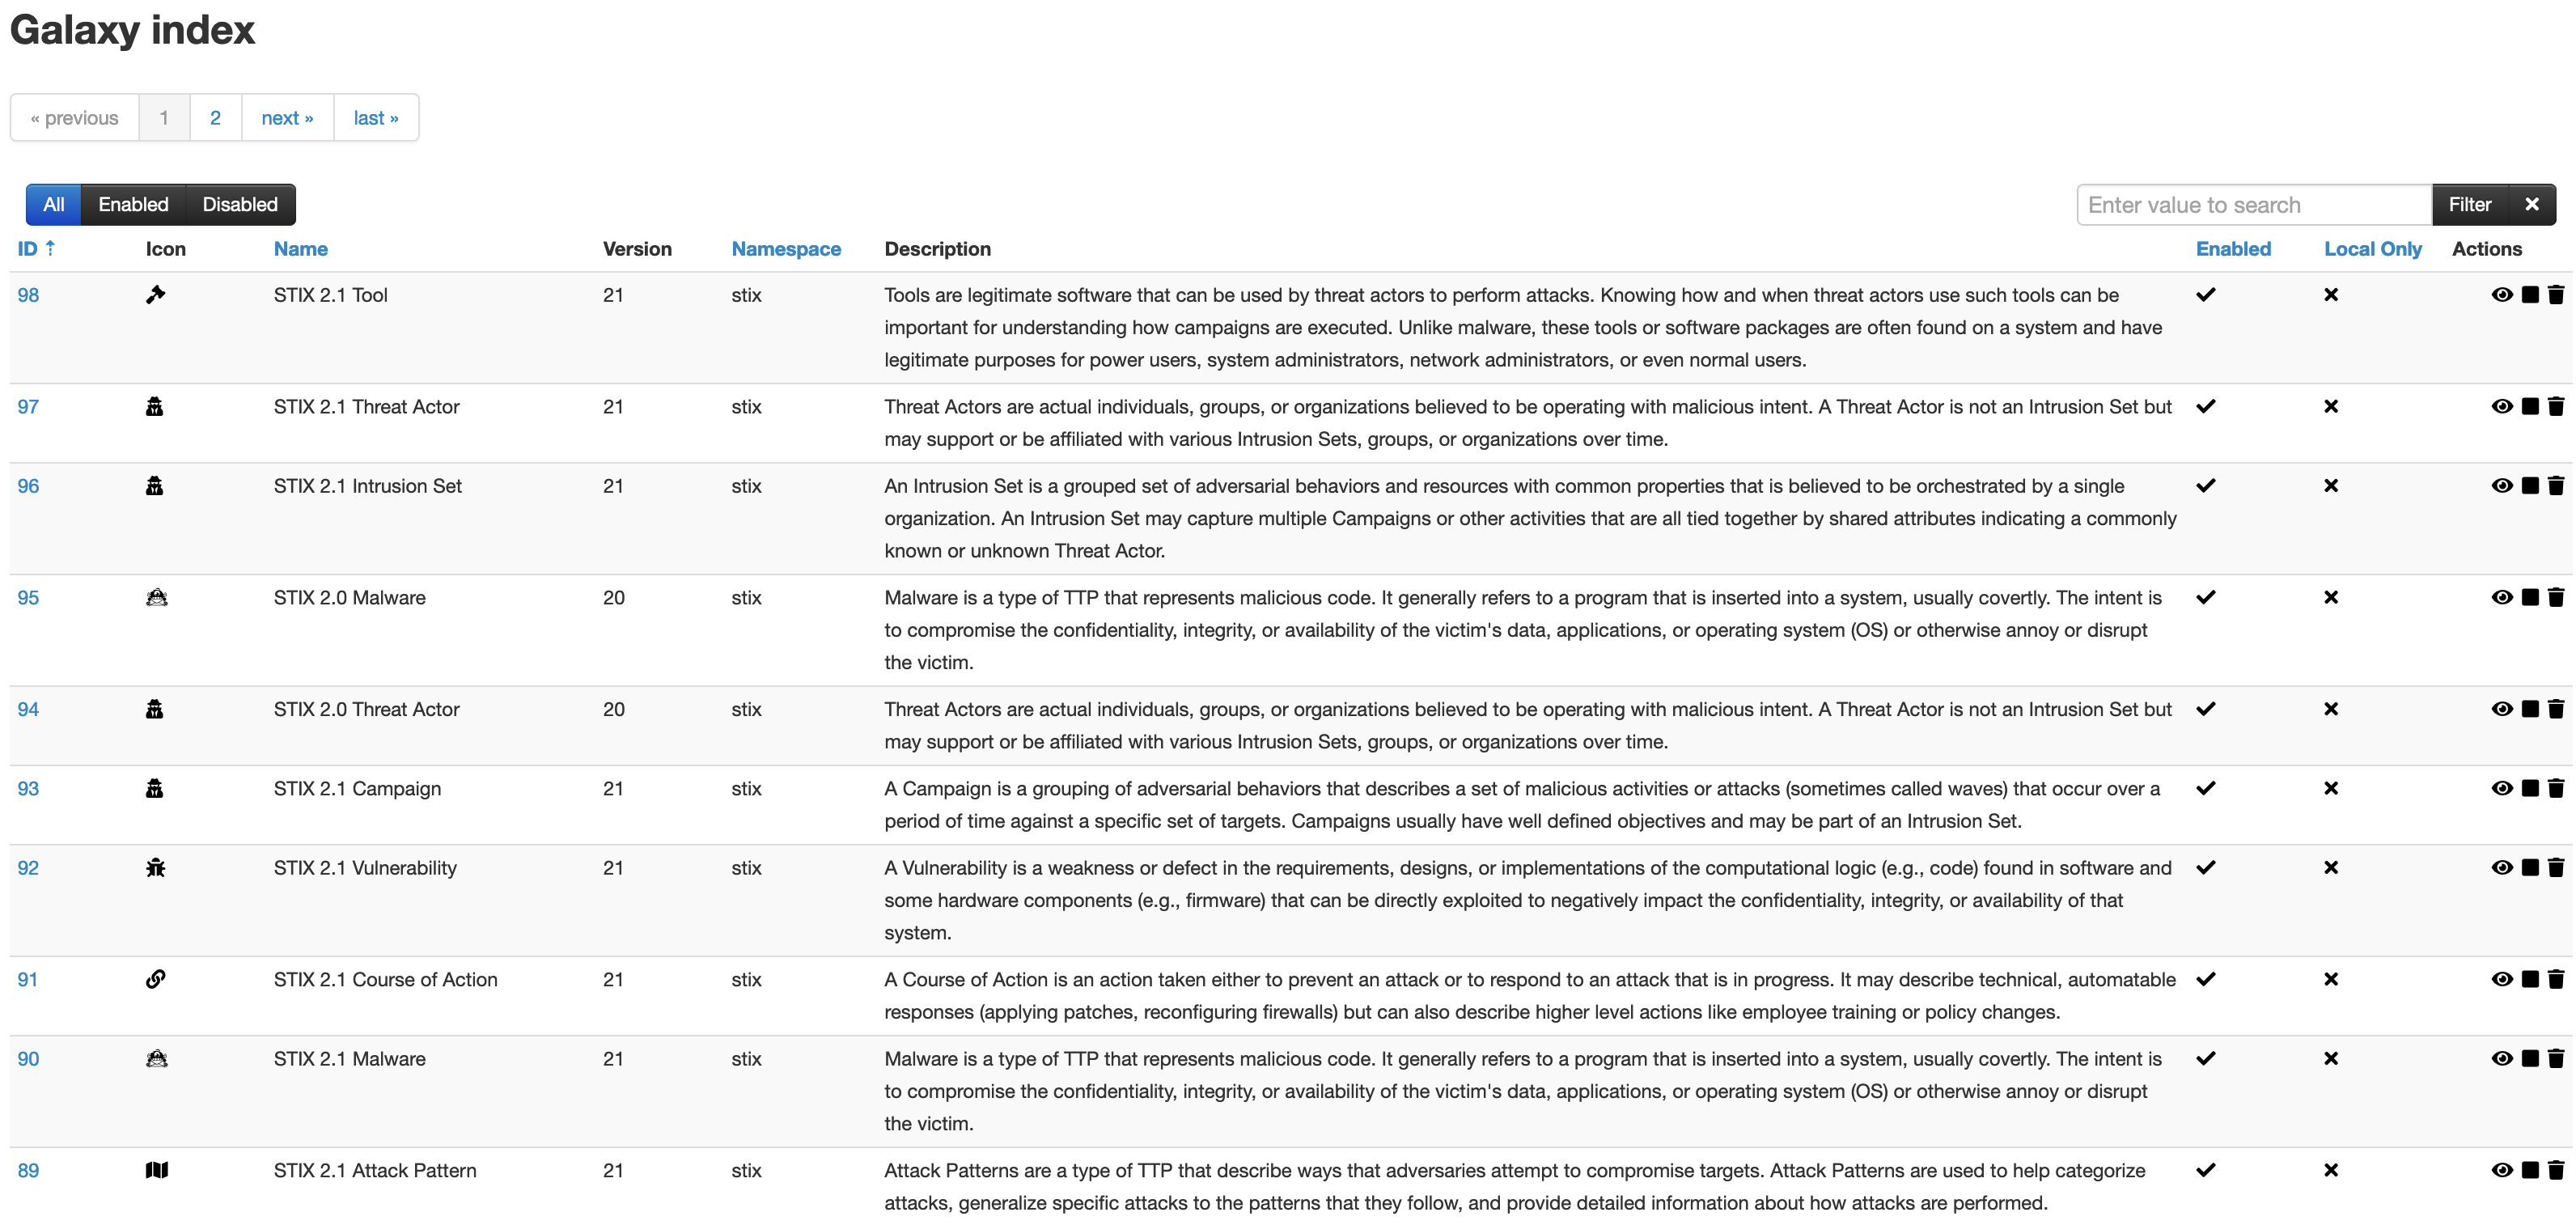
\includegraphics[scale=0.1]{stix-cluster.png}
	  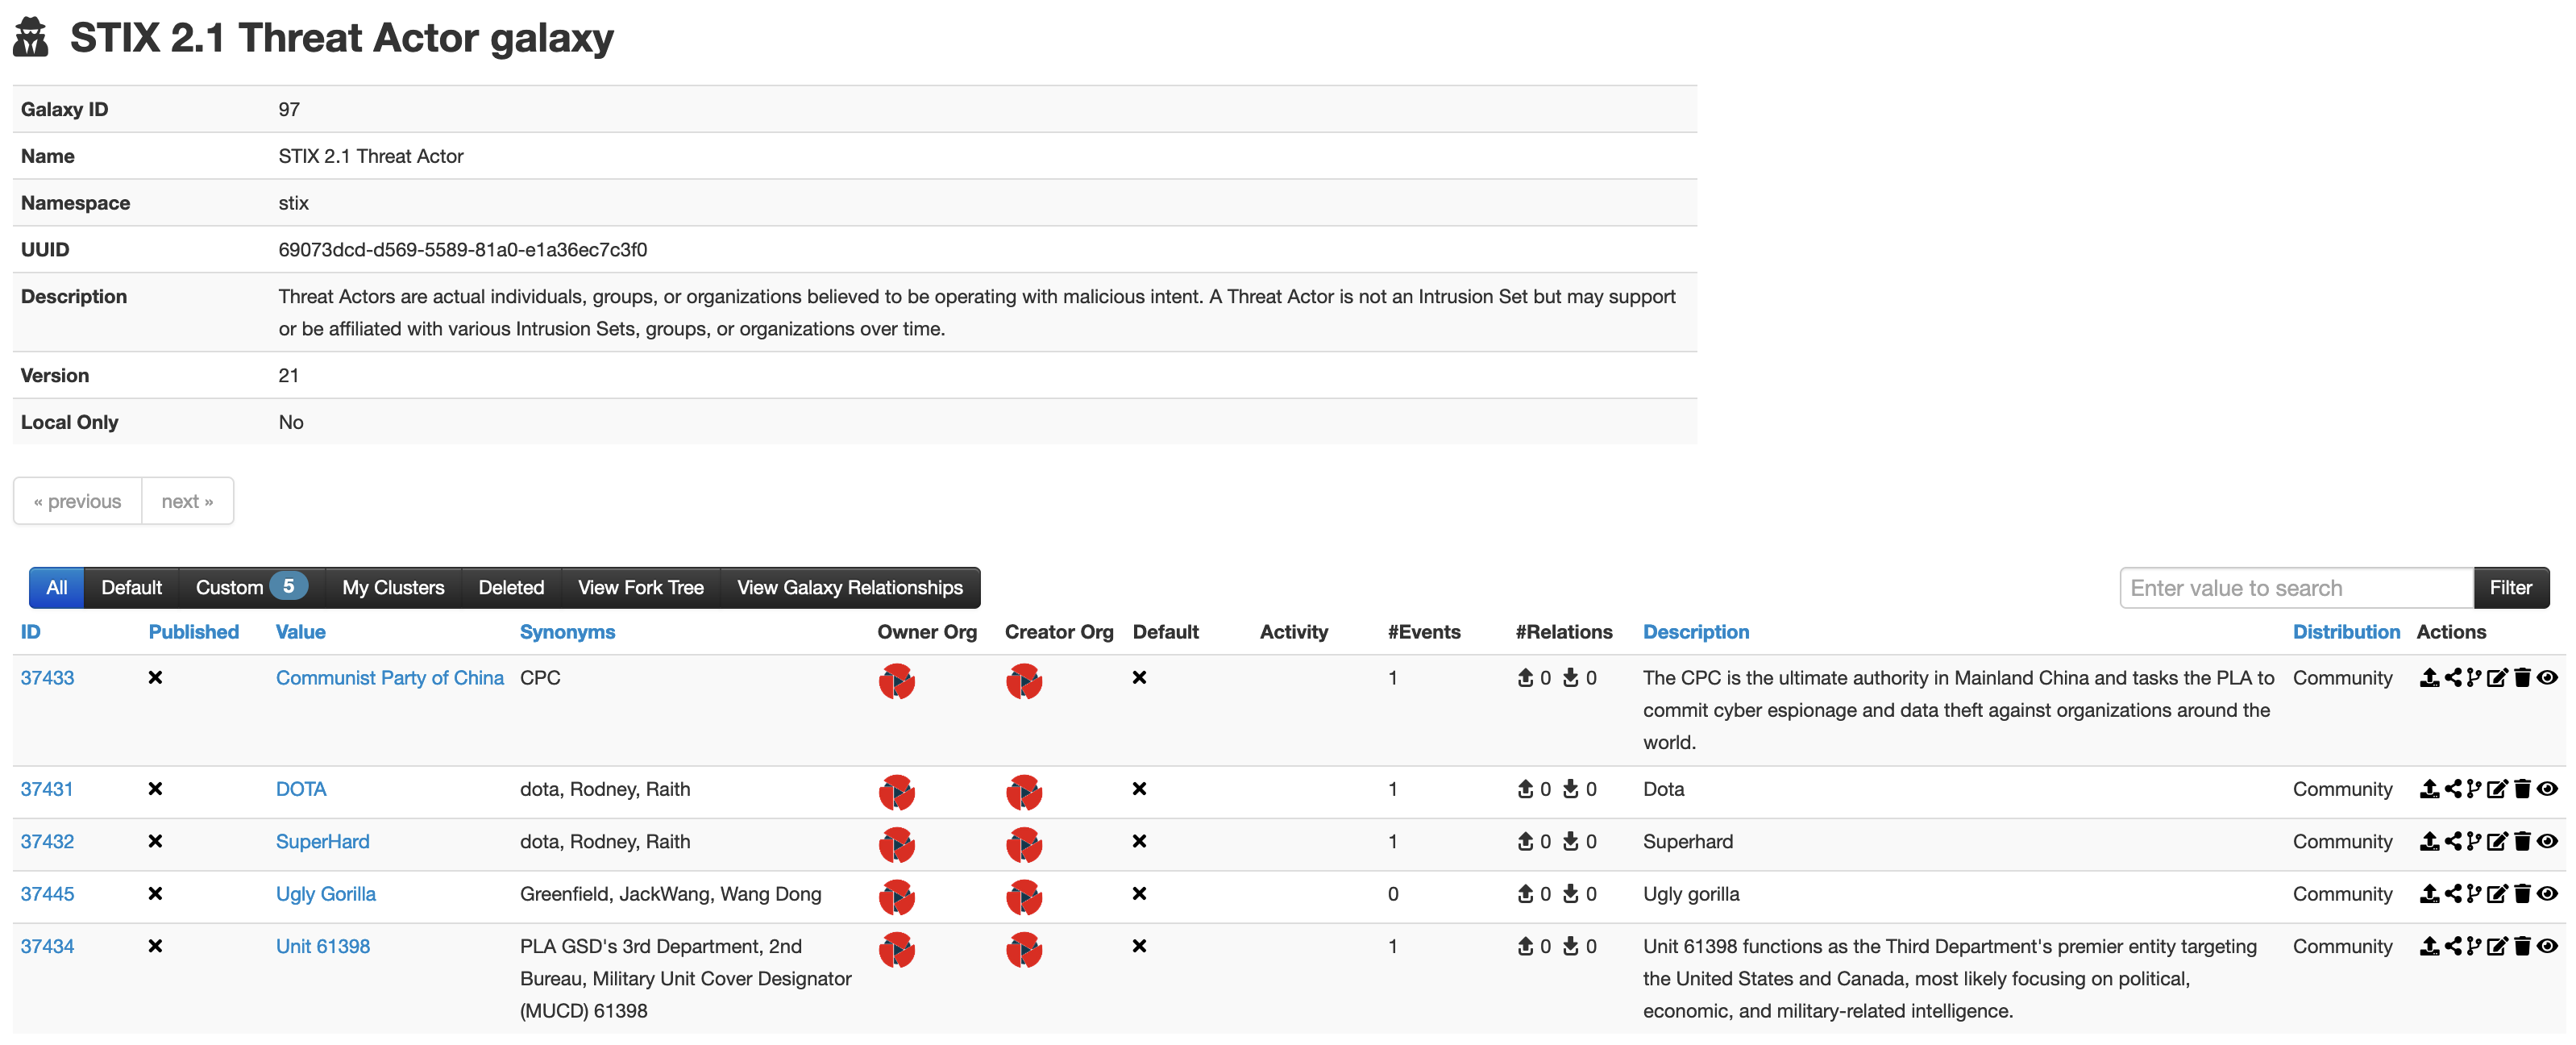
\includegraphics[scale=0.1]{stix-cluster2.png}
     \end{center}
\end{frame}

\begin{frame}
     \frametitle{MISP stix - Custom Galaxy Cluster Import}
     \begin{itemize}
        \item Extracting the complete description within the Cluster meta fields
	\begin{center}
	   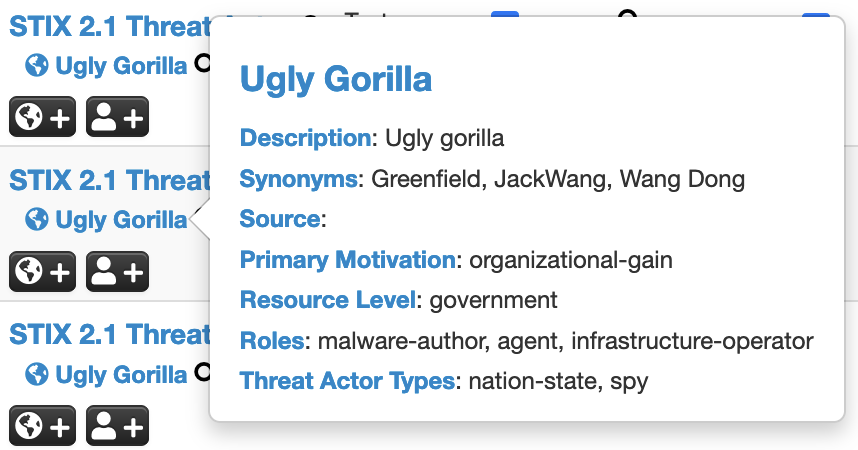
\includegraphics[scale=0.5]{stix-cluster3.png}
        \end{center}
     \end{itemize}
\end{frame}

\begin{frame}
     \frametitle{MISP stix - Distribution and MISP Galaxy 2.0}
     \begin{itemize}
        \item Ability to select the Clusters distribution
     \end{itemize}
	\begin{center}
	    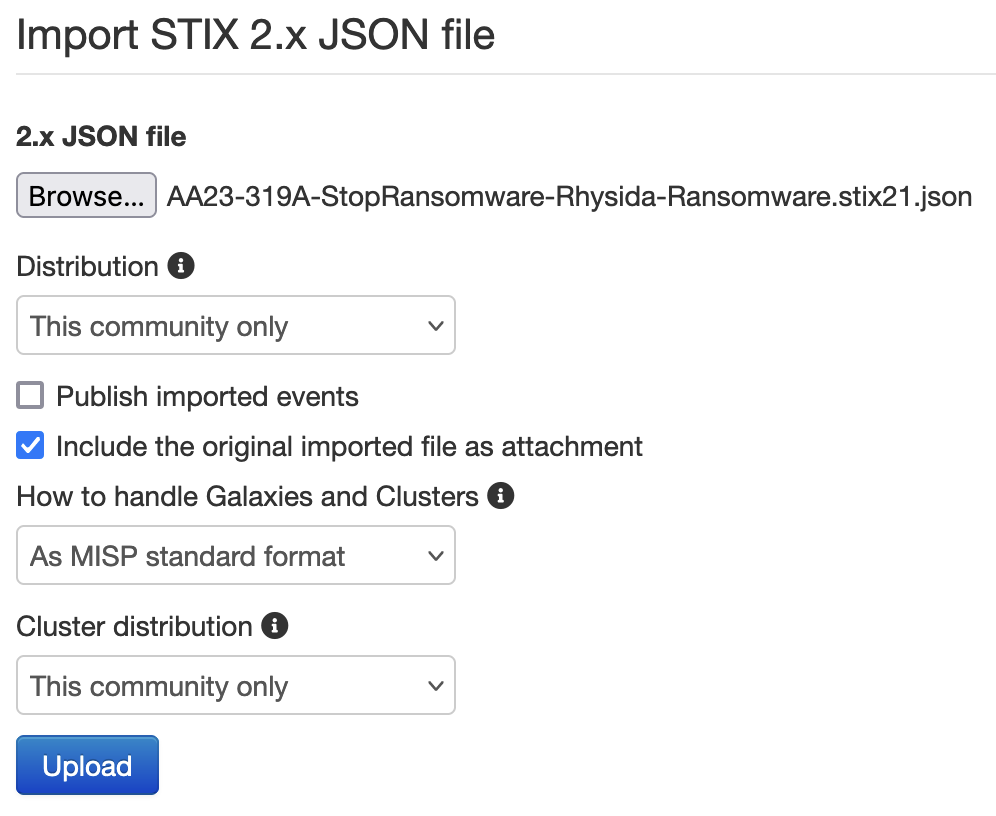
\includegraphics[scale=0.5]{stix-cluster4.png}
	\end{center}
\end{frame}

\begin{frame}
     \frametitle{MISP stix - Support of ACS markings}
     \begin{itemize}
	     \item Generating a {\bf Custom Galaxy Cluster} with the flattened description of the the Marking definition
             \item Extracting some of the fields as Tag to provide classification of the data marked with the Marking definition
     \end{itemize}
	\begin{center}
	    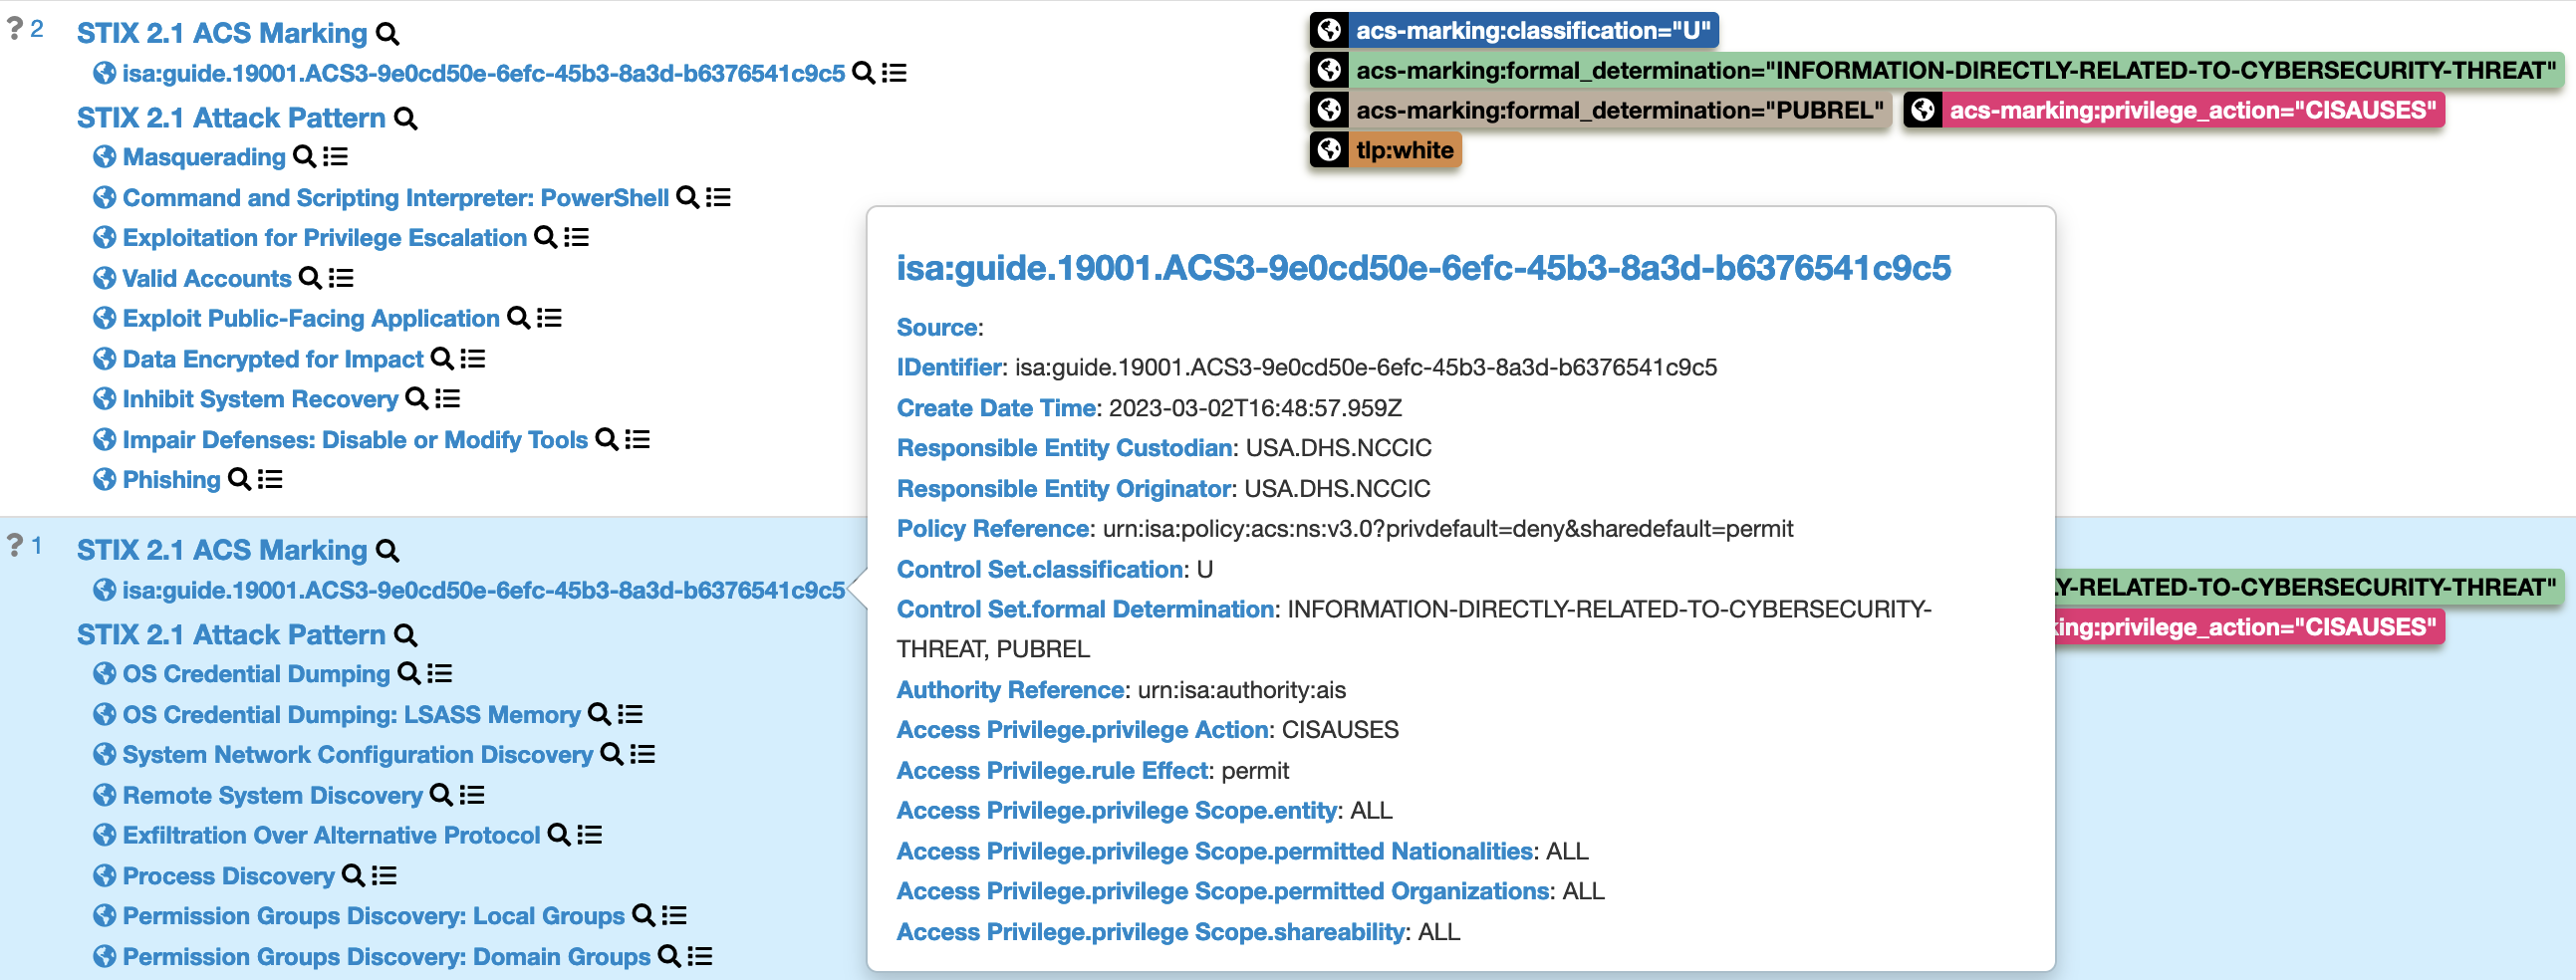
\includegraphics[scale=0.4]{stix-cluster5.png}
        \end{center}
\end{frame}

\begin{frame}
       \frametitle{Continuous improvement \& Work in progress}
	\begin{itemize}
		\item Import {\bf Note \& Opinion} objects using the recently released {\bf Analyst Data} feature
		\item Filling the mapping gaps between {\bf Indicators, Observed Data, Observable objects} and their MISP representation ({\bf Attributes \& Objects})
	\end{itemize}
\end{frame}

\begin{frame}
    \frametitle{Cerebrate}
    \begin{itemize}
        \item New documentation for Cerebrate\footnote{\url{https://doc.cerebrate-project.org/}}
        \item Many {\bf improvements and bugs fixed} following the feedback of different organisations deploying Cerebrate
        \item Deployment of the {\bf PoC for NATO users is ongoing}
        \item Software stack of MISP 3 is tested on Cerebrate
    \end{itemize}

\end{frame}

\section{Ongoing rework}

\begin{frame}
  \frametitle{MISP 3}
  \begin{itemize}
     \item Largest ongoing work is the work on {\bf MISP3}
     \item Already announced long ago, development is now underway\footnote{\url{https://github.com/MISP/MISP/tree/3.x}}
     \item New {\bf tech stack} based on Cerebrate's advances (CakePHP 4.x+, PHP 8.2+, Bootstrap 5+)
     \item Longer project, will bring long needed improvements
  \end{itemize}
\end{frame}

\section{MISP 3 Status}

\begin{frame}
	\frametitle{3.x Migration status}
	\begin{itemize}
	\item Migration status is available online in the MISP project page on GitHub\footnote{\url{https://github.com/orgs/MISP/projects/2/views/4}}
	\end{itemize}
	\begin{center}
		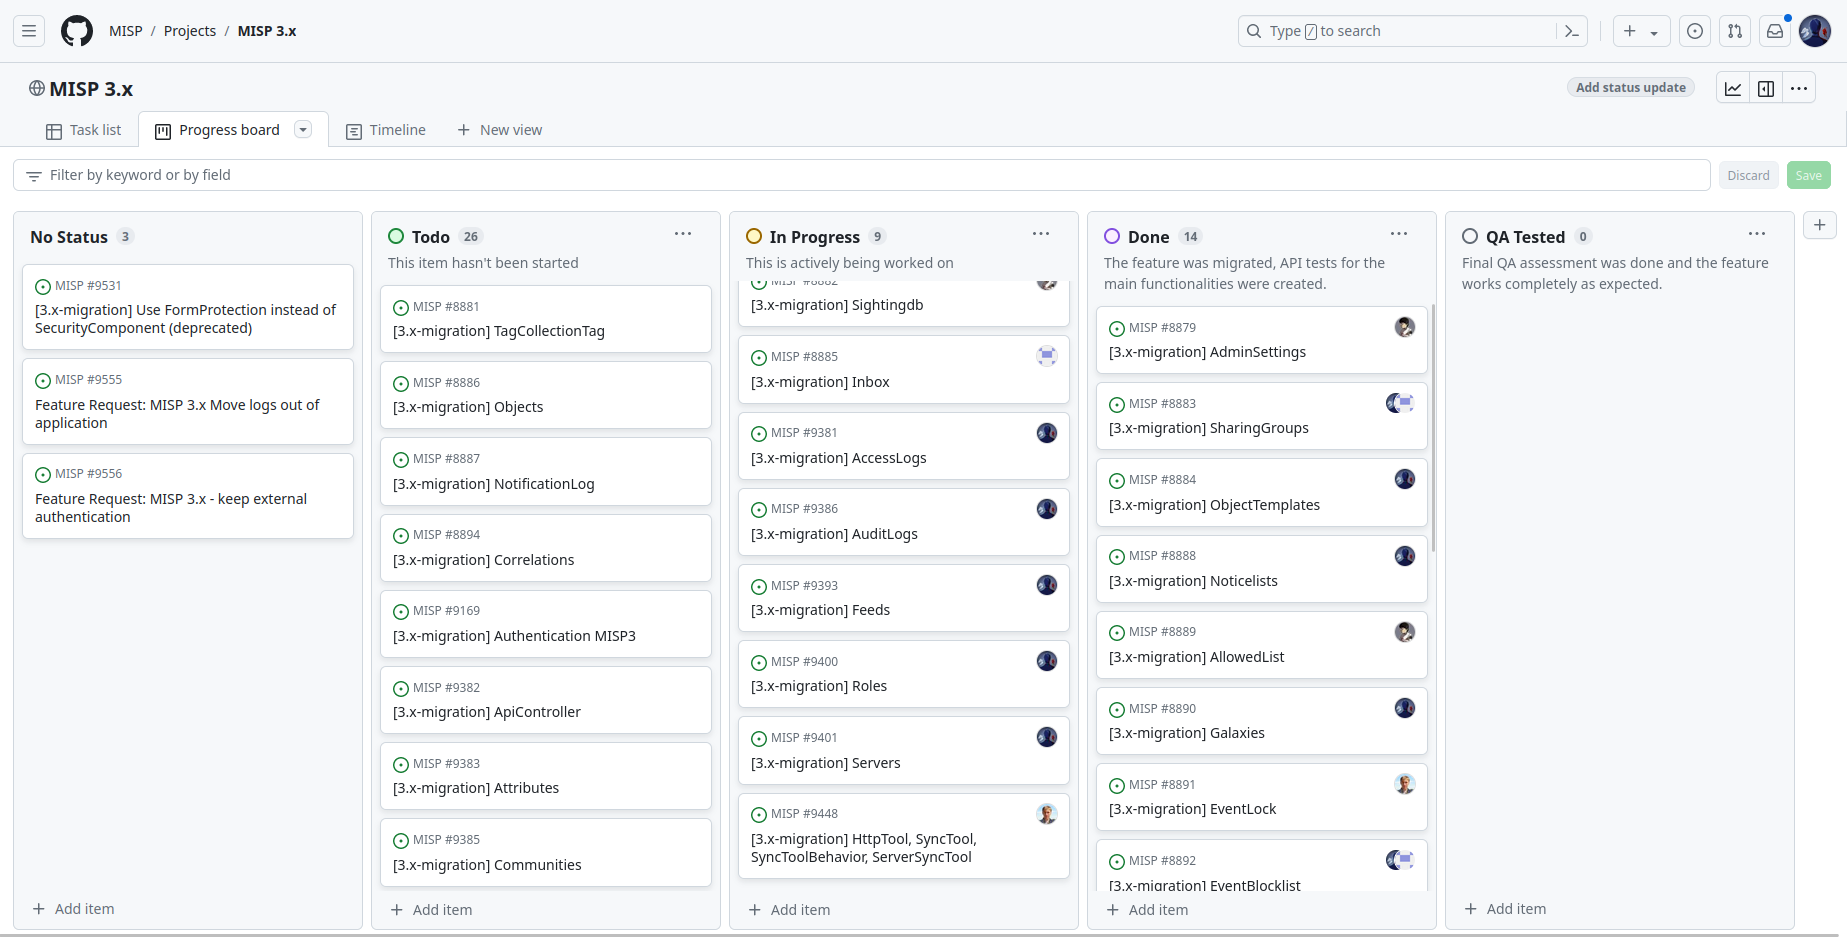
\includegraphics[scale=0.12]{misp3-project.png}
	\end{center}
	\begin{itemize}
		\item 26 Pull Requests (1 Open, 1 Draft)
		\item {\bf +105,165 lines of code added} and {\bf 20,992 lines of code removed}
	\end{itemize}
\end{frame}

\begin{frame}
        \frametitle{3.x - UI revamp}
	\begin{itemize}
	    \item {\bf Event View Page Redesign} - We are working on a complete overhaul of this page, with a focus on catering to multiple use-cases for different user-personas, enhancing responsiveness, integrating multiple charts, and emphasizing critical elements of MISP events. We’re also separating attributes and objects for clearer comprehension.
	    \item {\bf Navigation Menu Redesign} - We’re restructuring the navigation menu for better organization, incorporating intuitive groupings, icons, and support for mobile devices through a hamburger menu.
	    \item {\bf Bootstrap Upgrade} - Moving from Bootstrap 2 to Bootstrap 4 ensures a more modern and adaptable framework.
	\end{itemize}
\end{frame}

\begin{frame}
        \frametitle{3.x - UI revamp}
	\begin{itemize}
		\item {\bf Application-Wide Color Schemes} - We’re introducing support for customizable color schemes, including the much-requested dark mode.
		\item {\bf Settings and Diagnostics Page Redesign} - These sections will undergo a makeover to improve usability, accessibility and make them less overwhelming.
		\item {\bf Removal of Deprecated Features} - We aim to focus MISP’s functionality on core capabilities, we’re eliminating deprecated features that are no longer actively used or supported. This includes functionalities like Discussions or Threads, News, Scheduled Tasks, and Populate Event from Template.
	\end{itemize}
\end{frame}

\begin{frame}
        \frametitle{3.x - UI example}
	\begin{center}
		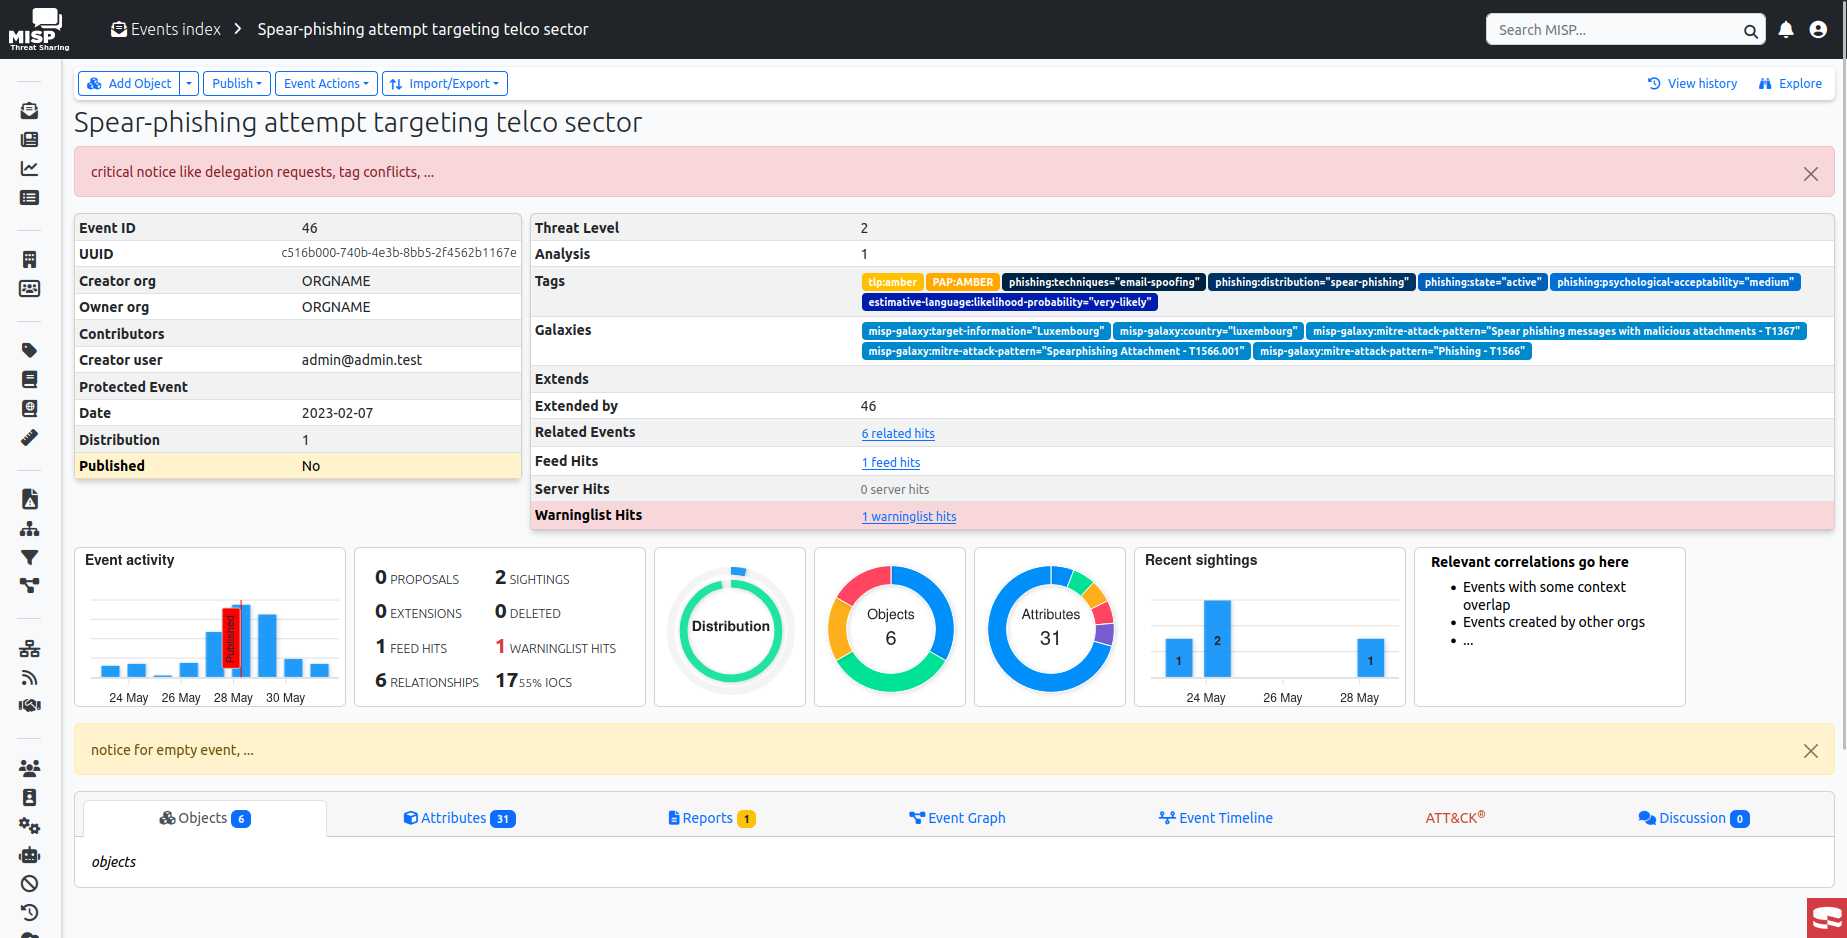
\includegraphics[scale=0.15]{misp3-ui.png}
	\end{center}
\end{frame}


\begin{frame}[fragile]
        \frametitle{3.x - Improved developer/deployment experience}
	\begin{itemize}
		\item Easy developer onboarding with dedicated readmes for development/testing.
		\item No more complex setup script, running docker development enviroment with just 3 commands:
	\end{itemize}
\begin{lstlisting}[basicstyle=\ttfamily\small, breaklines=true]
$ git clone -b 3.x git@github.com:MISP/MISP.git MISP3
$ cd MISP3
$ docker-compose -f docker-compose.yml -f docker-compose.dev.yml --env-file="./docker/.env.dev" up
\end{lstlisting}
\end{frame}

\begin{frame}
        \frametitle{3.x - Automatic checks/fixes via via pre-commit hooks}
	\begin{itemize}
		\item {\bf phpcbf}: Code style beautifying.
		\item {\bf phpcs}: Code style analysis PSR, naming conventions, etc.
		\item {\bf phpstan}: Automatic static code analysis unused variables/imports, forbidden functions, etc.
	\end{itemize}
\end{frame}

\begin{frame}[fragile]
	\frametitle{3.x - New test suite}
	\begin{itemize}
		\item Automatic API schema tests on requests/responses against OpenAPI spec.
		\item Code coverage.
		\item Testing sync and complex features mocking external http requests.
		\item Faster than previous PyMISP test suite.
		\item Reproducible, same tests are run by GitHub Actions on each PR.
		\item Easy to run, just one command:
	\end{itemize}
	\begin{lstlisting}[basicstyle=\ttfamily\small, breaklines=true,]
docker-compose -f docker-compose.yml -f docker-compose.dev.yml --env-file="./docker/.env.test" exec misp vendor/bin/phpunit
	\end{lstlisting}
\end{frame}

\begin{frame}
  \frametitle{MISP playbooks}
  \begin{itemize}
    \item A new project called MISP playbooks\footnote{\url{https://www.github.com/MISP/misp-playbooks}} has started
    \item MISP playbooks address {\bf common use-cases} encountereted by {\bf SOCs, CSIRTs and CTI teams}
    \item Covering all the activity such {\bf detecting, reacting and analysing}
    \item Documentation in Markdown format and code in Python all in {\bf Jupyter notebooks}
  \end{itemize}
\end{frame}

\begin{frame}
    \frametitle{MISP guard}
    \begin{itemize}
        \item misp-guard\footnote{\url{https://github.com/MISP/misp-guard}} is a mitmproxy addon that inspects the synchronization traffic (via PUSH or PULL) between different MISP instances and applies a set of customizable rules defined in a JSON file
        \item {\bf Simple code base for doing complementary filtering} between different MISPs for sensitive or classified networks
        \item misp-guard doesn't depend on MISP to apply the filtering
        \item Next step code review and evaluate the different option for certification (ideas are welcome)
    \end{itemize}
\end{frame}

\section{Conclusions}

\begin{frame}
  \frametitle{To sum it all up...}
  \begin{itemize}
     \item The MISP {\bf developer/contributor community} continues to grow and is very active
     \item The main focus the past year was on the following
     \begin{itemize}
          \item Performance, security, UX improvements
          \item Customisations of workflow processes
          \item Better operationalisation of MISP (community management, integration, monitoring)
          \item Fleshing out the documentation and supporting materials
     \end{itemize}
     \item Cerebrate is aiming to fill the void of community/fleet management that we currently have
     \item Definitely no lack of new ideas and improvements, if you want to participate, it's easy to {\bf get involved}
     \item Prioritisation is hard. {\bf Let us know what you think we should focus on}!
  \end{itemize}
\end{frame}

\begin{frame}
  \frametitle{Get in touch if you have any questions}
  \begin{itemize}
    \item Contact CIRCL
    \begin{itemize}
      \item info@circl.lu
      \item \url{https://social.circl.lu/@circl}
      \item \url{https://www.circl.lu/}
    \end{itemize}
    \item Contact MISPProject 
    \begin{itemize}
      \item \url{https://github.com/MISP}
      \item \url{https://gitter.im/MISP/MISP}
      \item \url{https://misp-community.org/@misp}
    \end{itemize}
    \item Cerebrate project
    \begin{itemize}
      \item \url{https://github.com/cerebrate-project}
      \item \url{https://github.com/cerebrate-project/cerebrate}
    \end{itemize}
  \end{itemize}
\end{frame}
